\documentclass[11pt]{article}\usepackage[]{graphicx}\usepackage[]{color}
%% maxwidth is the original width if it is less than linewidth
%% otherwise use linewidth (to make sure the graphics do not exceed the margin)
\makeatletter
\def\maxwidth{ %
  \ifdim\Gin@nat@width>\linewidth
    \linewidth
  \else
    \Gin@nat@width
  \fi
}
\makeatother

\definecolor{fgcolor}{rgb}{0.345, 0.345, 0.345}
\newcommand{\hlnum}[1]{\textcolor[rgb]{0.686,0.059,0.569}{#1}}%
\newcommand{\hlstr}[1]{\textcolor[rgb]{0.192,0.494,0.8}{#1}}%
\newcommand{\hlcom}[1]{\textcolor[rgb]{0.678,0.584,0.686}{\textit{#1}}}%
\newcommand{\hlopt}[1]{\textcolor[rgb]{0,0,0}{#1}}%
\newcommand{\hlstd}[1]{\textcolor[rgb]{0.345,0.345,0.345}{#1}}%
\newcommand{\hlkwa}[1]{\textcolor[rgb]{0.161,0.373,0.58}{\textbf{#1}}}%
\newcommand{\hlkwb}[1]{\textcolor[rgb]{0.69,0.353,0.396}{#1}}%
\newcommand{\hlkwc}[1]{\textcolor[rgb]{0.333,0.667,0.333}{#1}}%
\newcommand{\hlkwd}[1]{\textcolor[rgb]{0.737,0.353,0.396}{\textbf{#1}}}%
\let\hlipl\hlkwb

\usepackage{framed}
\makeatletter
\newenvironment{kframe}{%
 \def\at@end@of@kframe{}%
 \ifinner\ifhmode%
  \def\at@end@of@kframe{\end{minipage}}%
  \begin{minipage}{\columnwidth}%
 \fi\fi%
 \def\FrameCommand##1{\hskip\@totalleftmargin \hskip-\fboxsep
 \colorbox{shadecolor}{##1}\hskip-\fboxsep
     % There is no \\@totalrightmargin, so:
     \hskip-\linewidth \hskip-\@totalleftmargin \hskip\columnwidth}%
 \MakeFramed {\advance\hsize-\width
   \@totalleftmargin\z@ \linewidth\hsize
   \@setminipage}}%
 {\par\unskip\endMakeFramed%
 \at@end@of@kframe}
\makeatother

\definecolor{shadecolor}{rgb}{.97, .97, .97}
\definecolor{messagecolor}{rgb}{0, 0, 0}
\definecolor{warningcolor}{rgb}{1, 0, 1}
\definecolor{errorcolor}{rgb}{1, 0, 0}
\newenvironment{knitrout}{}{} % an empty environment to be redefined in TeX

\usepackage{alltt}
%\usepackage[showframe]{geometry}
\usepackage[table]{xcolor}
\usepackage{caption}
\usepackage{lscape,verbatim,mathrsfs}
\usepackage{graphics,amsmath,pstricks}
\usepackage{amssymb,enumerate}
\usepackage{amsbsy,amsmath,amsthm,amsfonts, amssymb}
\usepackage{graphicx, rotate, array}
\usepackage{geometry,multirow}
\usepackage{color,soul}
\usepackage{float}
%\usepackage{hyperref}
\usepackage[authoryear,round]{natbib}
%\renewcommand{\baselinestretch}{1.9}
\usepackage{tcolorbox}
\renewcommand{\familydefault}{cmss}
\textwidth=6.65in \textheight=9.7in
\parskip=.025in
\parindent=0in
\oddsidemargin=-0.1in \evensidemargin=-.1in \headheight=-.6in
\footskip=0.5in \DeclareMathOperator*{\argmax}{argmax}
\DeclareMathOperator*{\argmin}{argmin}
\IfFileExists{upquote.sty}{\usepackage{upquote}}{}
\begin{document}









SMOOTH2






\begin{knitrout}
\definecolor{shadecolor}{rgb}{0.969, 0.969, 0.969}\color{fgcolor}
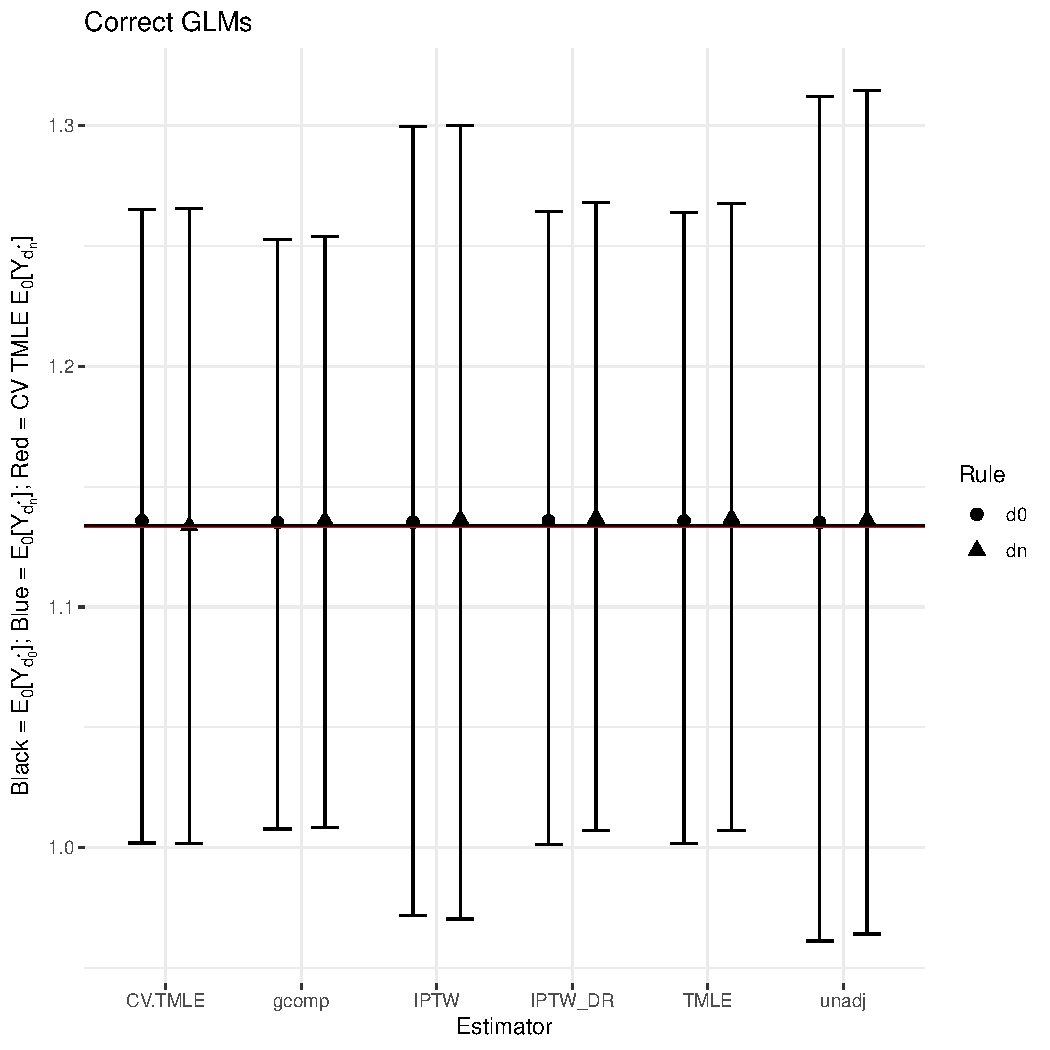
\includegraphics[width=\maxwidth]{figure/unnamed-chunk-1-1} 

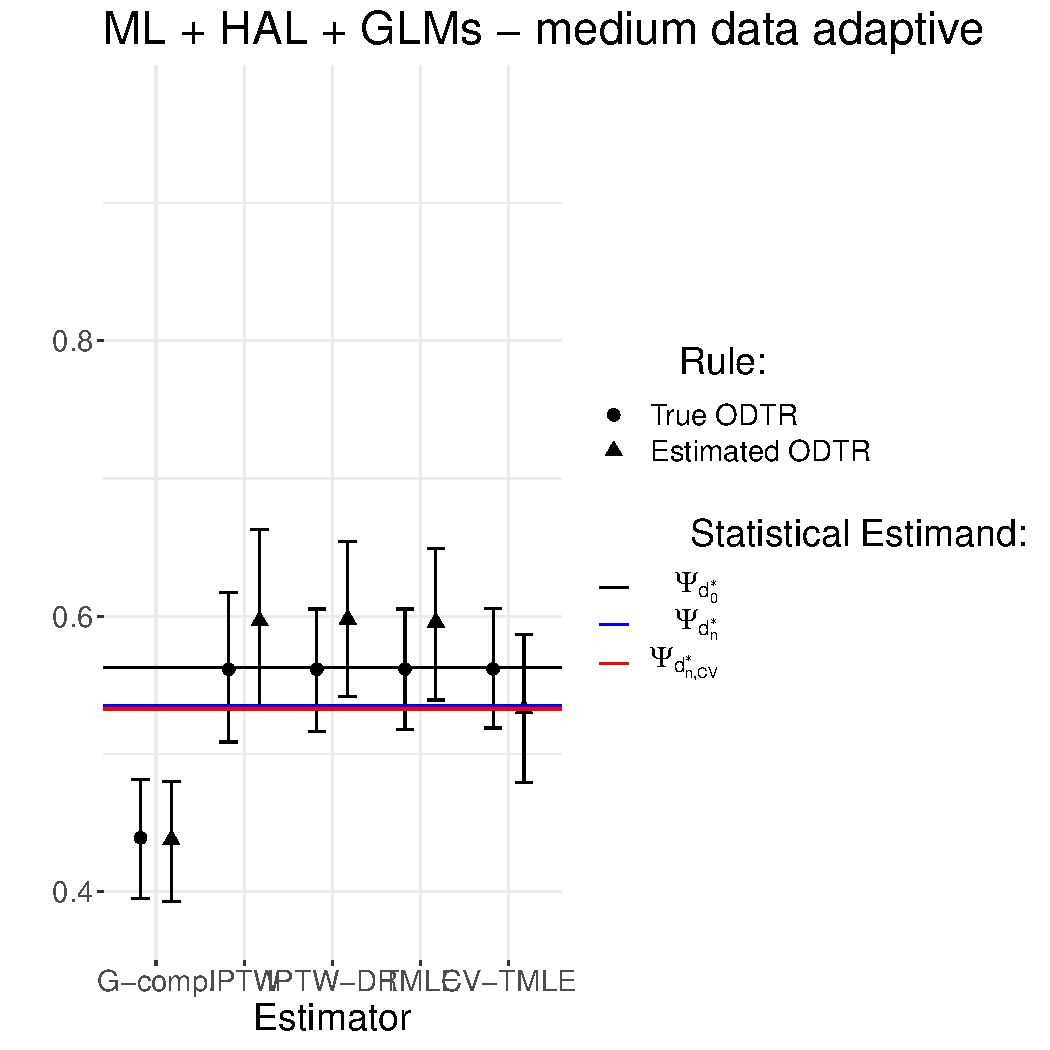
\includegraphics[width=\maxwidth]{figure/unnamed-chunk-1-2} 

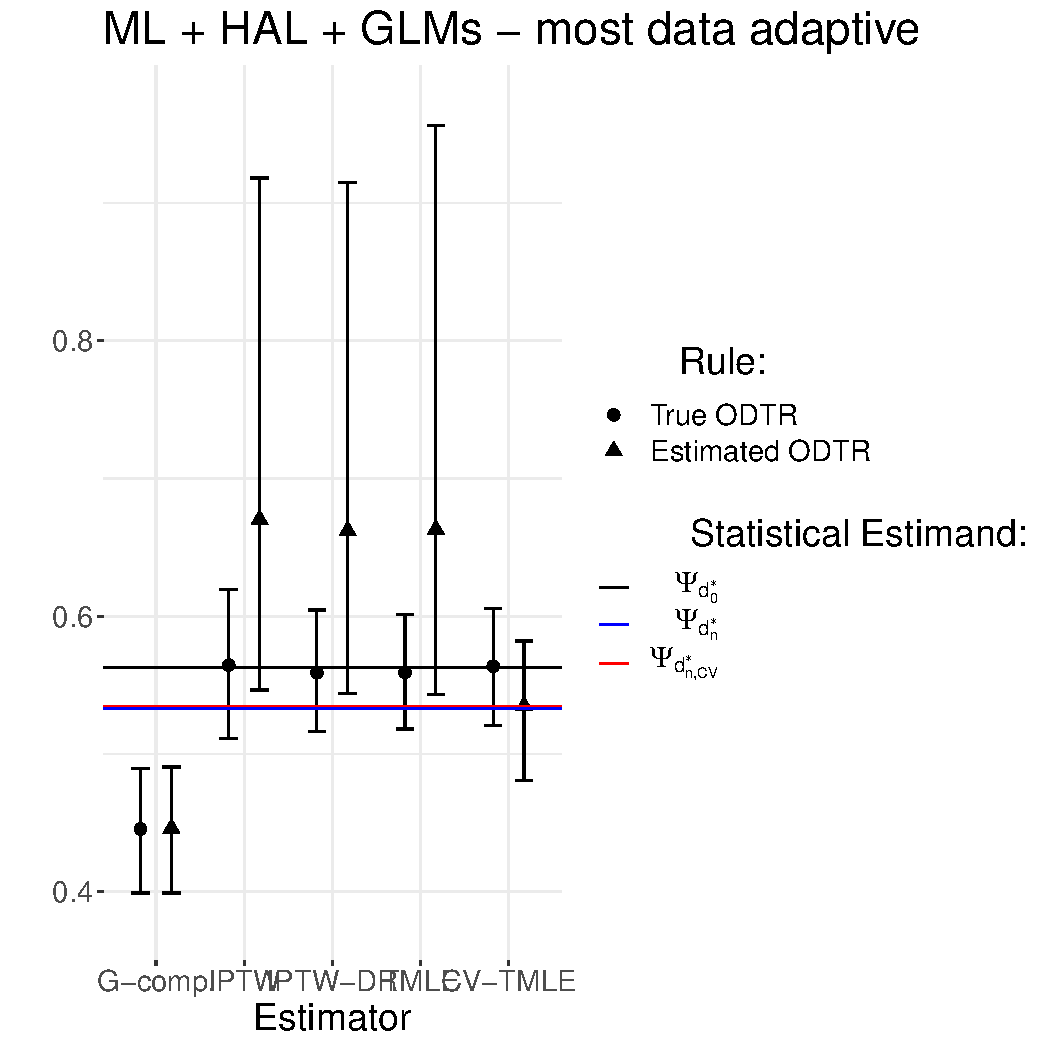
\includegraphics[width=\maxwidth]{figure/unnamed-chunk-1-3} 

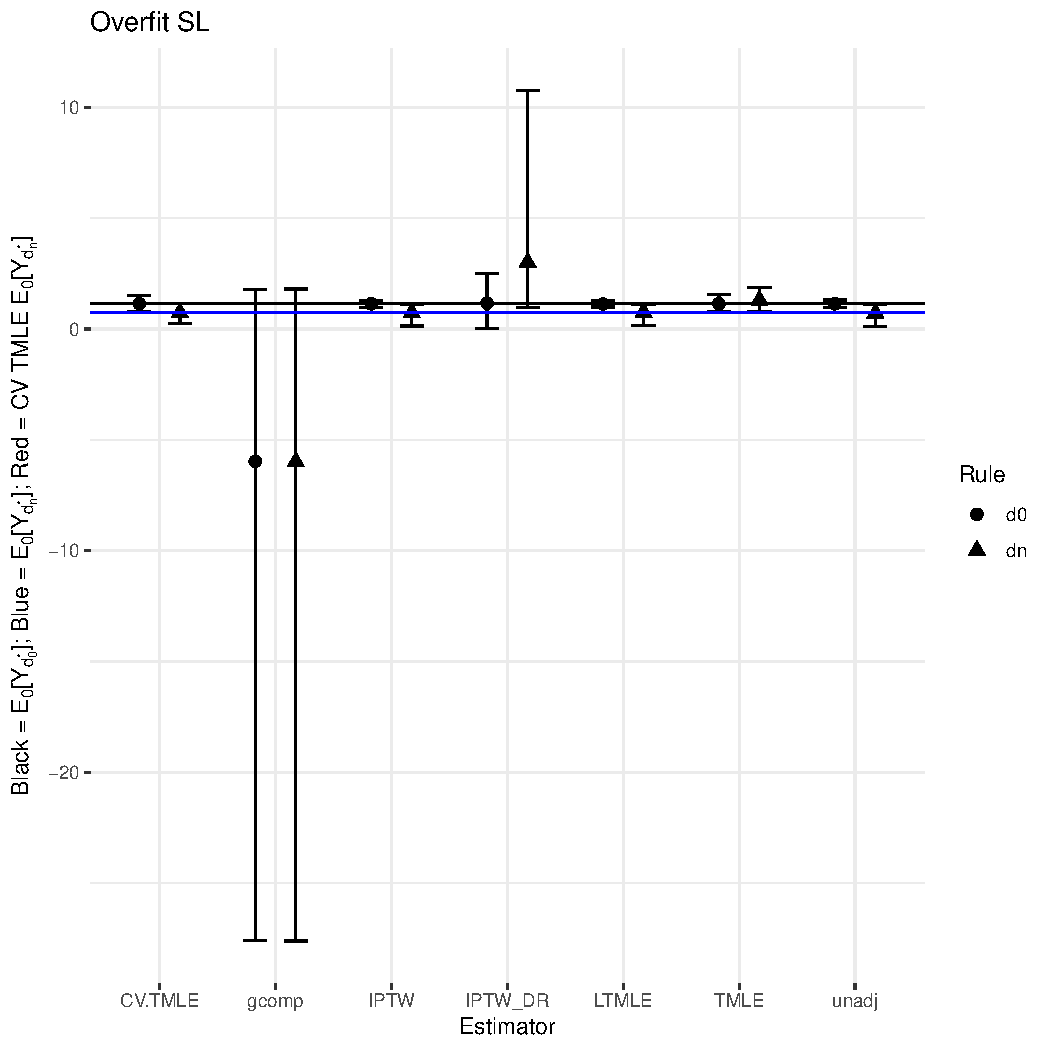
\includegraphics[width=\maxwidth]{figure/unnamed-chunk-1-4} 

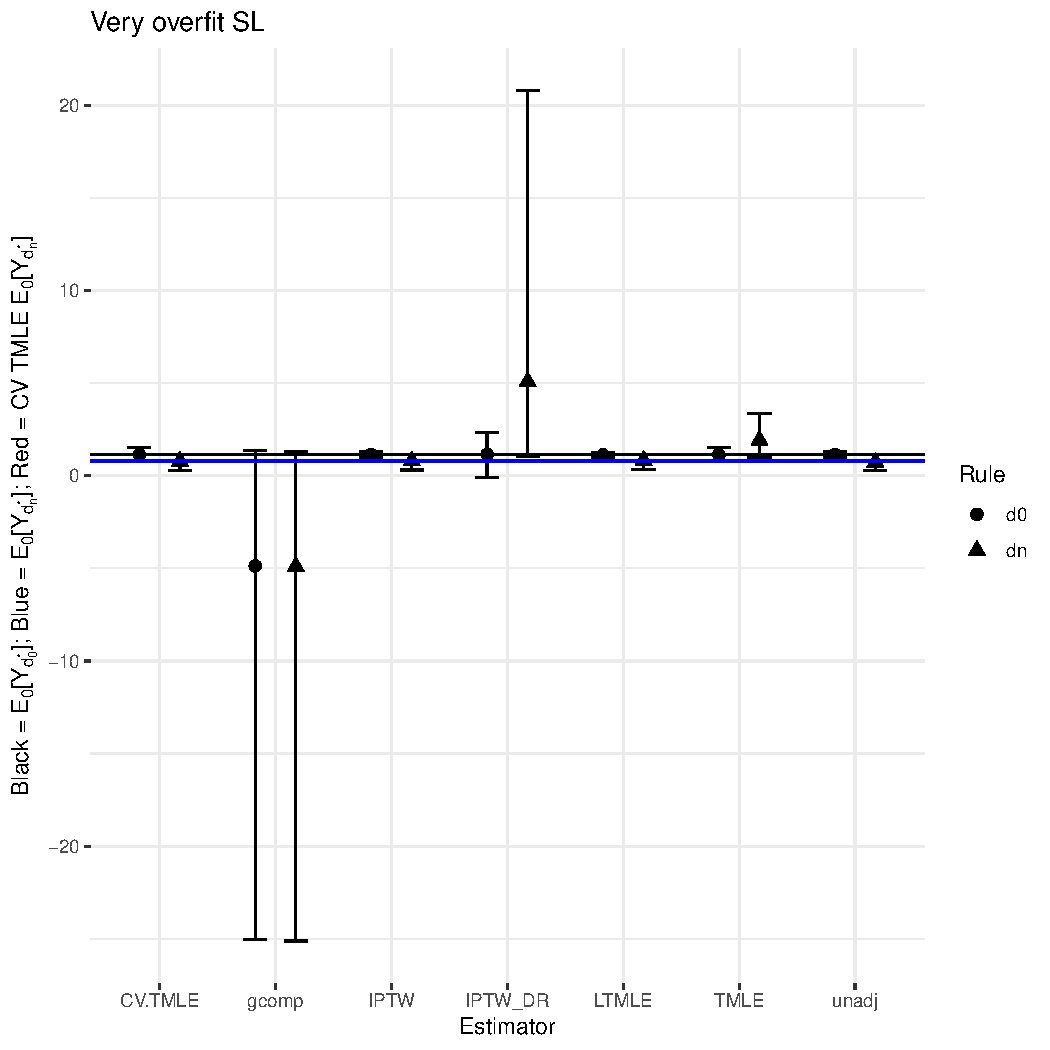
\includegraphics[width=\maxwidth]{figure/unnamed-chunk-1-5} 

\end{knitrout}



\begin{knitrout}
\definecolor{shadecolor}{rgb}{0.969, 0.969, 0.969}\color{fgcolor}\begin{kframe}
\begin{alltt}
\hlcom{# Correct GLM}
\hlkwd{make_table_EYdopt}\hlstd{(}\hlkwc{EYdopt} \hlstd{= EYdopt_step1_smooth2,} \hlkwc{truevalues} \hlstd{= DGP_smooth2_true_values)}
\end{alltt}
\begin{verbatim}
##                    Bias Variance    MSE Coverage
## unadj            0.0023   0.0081 0.0081    0.995
## gcomp             0.002   0.0041 0.0041        -
## IPTW             0.0024    0.007  0.007     0.97
## IPTW_DR          0.0029   0.0045 0.0045    0.958
## TMLE             0.0028   0.0045 0.0045    0.956
## LTMLE                 -        -      -        -
## CV.TMLE          -3e-04   0.0046 0.0046    0.952
## unadj_dopt0      0.0011   0.0081 0.0081    0.995
## gcomp_dopt0      0.0011   0.0041 0.0041        -
## IPTW_dopt0       0.0013   0.0071 0.0071    0.967
## IPTW_DR_dopt0    0.0018   0.0046 0.0046    0.955
## TMLE_dopt0       0.0018   0.0046 0.0046    0.956
## LTMLE_dopt0           -        -      -        -
## CV.TMLE_dopt0    0.0018   0.0046 0.0046    0.955
## unadj_sampspec   0.0025   0.0081  0.005        1
## gcomp_sampspec   0.0022   0.0041 0.0015        -
## IPTW_sampspec    0.0026    0.007 0.0041    0.994
## IPTW_DR_sampspec 0.0031   0.0045  0.002    0.997
## LTMLE_sampspec        -        -      -        -
## TMLE_sampspec    0.0031   0.0045  0.002    0.997
## CV.TMLE_sampspec  2e-04   0.0046  0.002    0.997
\end{verbatim}
\begin{alltt}
\hlcom{# Incorrect GLM}
\hlkwd{make_table_EYdopt}\hlstd{(}\hlkwc{EYdopt} \hlstd{= EYdopt_step2_smooth2,} \hlkwc{truevalues} \hlstd{= DGP_smooth2_true_values)}
\end{alltt}
\begin{verbatim}
##                     Bias Variance    MSE Coverage
## unadj            -0.3676   0.0108 0.1459    0.158
## gcomp            -0.3678   0.0077  0.143        -
## IPTW              -0.367   0.0092 0.1439    0.052
## IPTW_DR          -0.3676   0.0083 0.1434     0.02
## TMLE             -0.3675   0.0083 0.1433    0.022
## LTMLE                  -        -      -        -
## CV.TMLE          -0.3853   0.0086 0.1571    0.013
## unadj_dopt0       0.0011   0.0081 0.0081    0.995
## gcomp_dopt0      -0.6294    0.007 0.4031        -
## IPTW_dopt0        0.0013   0.0071 0.0071    0.967
## IPTW_DR_dopt0    -0.0017   0.0056 0.0056    0.955
## TMLE_dopt0             0   0.0054 0.0054     0.95
## LTMLE_dopt0            -        -      -        -
## CV.TMLE_dopt0     0.0023   0.0055 0.0055     0.95
## unadj_sampspec     0.008   0.0108 0.0062    0.999
## gcomp_sampspec    0.0078   0.0077 0.0039        -
## IPTW_sampspec     0.0087   0.0092 0.0051    0.994
## IPTW_DR_sampspec  0.0081   0.0083 0.0042    0.988
## LTMLE_sampspec         -        -      -        -
## TMLE_sampspec     0.0081   0.0083 0.0042    0.987
## CV.TMLE_sampspec -0.0027   0.0086 0.0041     0.99
\end{verbatim}
\begin{alltt}
\hlcom{# Non-overfit SL}
\hlkwd{make_table_EYdopt}\hlstd{(}\hlkwc{EYdopt} \hlstd{= EYdopt_step3_smooth2,} \hlkwc{truevalues} \hlstd{= DGP_smooth2_true_values)}
\end{alltt}
\begin{verbatim}
##                     Bias Variance    MSE Coverage
## unadj            -0.3641   0.0092 0.1417    0.145
## gcomp            -0.9701   0.0438 0.9848        -
## IPTW             -0.3642   0.0086 0.1412    0.045
## IPTW_DR          -0.3647   0.0082 0.1412    0.027
## TMLE             -0.3636   0.0079 0.1401    0.018
## CV.TMLE          -0.3876   0.0083 0.1586    0.012
## unadj_dopt0       0.0027   0.0072 0.0072    0.998
## gcomp_dopt0      -0.9759   0.0418 0.9942        -
## IPTW_dopt0        0.0034   0.0068 0.0068    0.975
## IPTW_DR_dopt0     0.0003   0.0061 0.0061    0.968
## TMLE_dopt0        0.0007   0.0053 0.0053    0.966
## CV.TMLE_dopt0     0.0031   0.0055 0.0055    0.967
## LTMLE            -0.3657   0.0076 0.1413     0.01
## LTMLE_dopt0       0.0006   0.0049 0.0049    0.965
## unadj_sampspec    0.0148   0.0092 0.0059        1
## gcomp_sampspec   -0.5912   0.0438 0.3931        -
## IPTW_sampspec     0.0147   0.0086 0.0052    0.996
## IPTW_DR_sampspec  0.0141   0.0082 0.0048    0.997
## LTMLE_sampspec    0.0131   0.0076 0.0041    0.996
## TMLE_sampspec     0.0152   0.0079 0.0046    0.995
## CV.TMLE_sampspec -0.0003   0.0083 0.0045    0.995
\end{verbatim}
\begin{alltt}
\hlkwd{make_table_EYdopt}\hlstd{(}\hlkwc{EYdopt} \hlstd{= EYdopt_step4_smooth2,} \hlkwc{truevalues} \hlstd{= DGP_smooth2_true_values)}
\end{alltt}
\begin{verbatim}
##                     Bias Variance      MSE Coverage
## unadj            -0.4233   0.0678   0.2469    0.325
## gcomp            -7.1219  72.3852 123.0346        -
## IPTW             -0.3980   0.0624   0.2207    0.212
## IPTW_DR           1.8747   7.3525  10.8597    0.379
## TMLE              0.1632   0.0766   0.1031    0.743
## CV.TMLE          -0.3994   0.0506   0.2101    0.411
## unadj_dopt0       0.0007   0.0076   0.0076    0.997
## gcomp_dopt0      -7.1046  72.2634 122.6658        -
## IPTW_dopt0        0.0006   0.0074   0.0073     0.97
## IPTW_DR_dopt0     0.0309   0.3670   0.3676    0.942
## TMLE_dopt0        0.0028   0.0335   0.0335    0.954
## CV.TMLE_dopt0     0.0024   0.0311   0.0310    0.944
## LTMLE            -0.3797   0.0656   0.2097     0.19
## LTMLE_dopt0      -0.0081   0.0053   0.0053    0.945
## unadj_sampspec   -0.0370   0.0678   0.0082    0.996
## gcomp_sampspec   -6.7356  72.3852 114.9904        -
## IPTW_sampspec    -0.0118   0.0624   0.0065    0.986
## IPTW_DR_sampspec  2.2610   7.3525  13.2520    0.171
## LTMLE_sampspec    0.0066   0.0656   0.0026    0.997
## TMLE_sampspec     0.5494   0.0766   0.4259     0.26
## CV.TMLE_sampspec -0.0054   0.0506   0.0315    0.944
\end{verbatim}
\begin{alltt}
\hlkwd{make_table_EYdopt}\hlstd{(}\hlkwc{EYdopt} \hlstd{= EYdopt_step5_smooth2,} \hlkwc{truevalues} \hlstd{= DGP_smooth2_true_values)}
\end{alltt}
\begin{verbatim}
##                     Bias Variance     MSE Coverage
## unadj            -0.4059   0.0568  0.2216    0.306
## gcomp            -6.0318  61.1617 97.4833        -
## IPTW             -0.3387   0.0484  0.1631    0.272
## IPTW_DR           3.9490  30.7465 46.3101    0.133
## TMLE              0.7811   0.5343  1.1439    0.222
## CV.TMLE          -0.3522   0.0487  0.1727    0.457
## unadj_dopt0       0.0018   0.0079  0.0078    0.996
## gcomp_dopt0      -6.0059  60.9575 96.9668        -
## IPTW_dopt0        0.0019   0.0071  0.0071    0.969
## IPTW_DR_dopt0     0.0118   0.3231  0.3229     0.94
## TMLE_dopt0       -0.0053   0.0328  0.0328    0.937
## CV.TMLE_dopt0     0.0009   0.0332  0.0332    0.938
## LTMLE            -0.3040   0.0549  0.1472    0.303
## LTMLE_dopt0      -0.0095   0.0051  0.0051    0.944
## unadj_sampspec   -0.0597   0.0568  0.0184    0.955
## gcomp_sampspec   -5.6855  61.1617 90.9031        -
## IPTW_sampspec     0.0076   0.0484  0.0135     0.91
## IPTW_DR_sampspec  4.2952  30.7465 50.8612    0.061
## LTMLE_sampspec    0.0423   0.0549  0.0057    0.948
## TMLE_sampspec     1.1274   0.5343  1.9671    0.078
## CV.TMLE_sampspec -0.0055   0.0487  0.0292    0.956
\end{verbatim}
\end{kframe}
\end{knitrout}


\end{document}
